% !TEX encoding = UTF-8 Unicode
\documentclass[a4paper]{article}

\usepackage{color}
\usepackage{url}
\usepackage[utf8]{inputenc} % make weird characters work
\usepackage{graphicx}
%\usepackage{caption}
%\usepackage[nottoc]{tocbibind}

\usepackage[serbian]{babel}

\usepackage{caption}
\usepackage{subcaption}

\usepackage{color}
\usepackage{listings}
\usepackage{setspace}

\usepackage{indentfirst}
\usepackage[unicode]{hyperref}
\hypersetup{colorlinks,citecolor=green,filecolor=green,linkcolor=blue,urlcolor=blue}

\usepackage{color}

\definecolor{mygreen}{rgb}{0,0.6,0}
\definecolor{mygray}{rgb}{0.5,0.5,0.5}
\definecolor{mymauve}{rgb}{0.58,0,0.82}

\begin{document}

\title{Klasifikacija centara najbolje petorke NBA lige}
\author{David Gavrilović}
% \date{...}
\maketitle
\thispagestyle{empty}

\newpage

\tableofcontents
\thispagestyle{empty}

\newpage

\section{Statistika 101}
\label{sec:stats_101}

U ovoj glavi ćemo su upoznati sa raznim košarkaškim statističkim statistikama. Postoje dve grupe, tradicionalna i napredna statistika.

\subsection{Tradicionalna statistika}
\label{subsec:trad_stat}

\begin{itemize}
	\item \textbf{Pos} - Pozicija igrača. Tradicionalno, igrač može biti: Plejmejker \textbf{PG}, Bek šuter \textbf{SG}, Nisko krilo \textbf{SF}, visoko krilo ili krilni centar \textbf{PF} ili centar \textbf{C}. U današnjoj košarci, jedan igrač može da igra na više pozicija i često je jedan od: \textbf{Point} - plejmejker, \textbf{Combo guard} - može biti plejmejker ili bek šuter, \textbf{Wing} - bek šuter ili nisko krilo, \textbf{Forward} - nisko ili visoko krilo, \textbf{Big} - najčešće centar, ali može biti i visoko krilo.
    \item \textbf{G} - Broj utakmica u kojima je igrač igrao u toku sezone.
    \item \textbf{GS} - Broj utakmica u kojima je igrač bio u startnoj petorci.
    \item \textbf{MP} - Odigrani minuti.
    \item \textbf{FG} - Broj pogođenih šuteva na koš iz igre.
    \item \textbf{FGA} - Broj pokušanih šuteva na koš.
    \item \textbf{FG\%} - Procenat pogođenih šuteva. Računa se kao FG / FGA.
    \item \textbf{3P} - Broj pogođenih šuteva za tri poena.
    \item \textbf{3PA} - Broj pokušanih šuteva za tri poena.
    \item \textbf{3P\%} - Procenat pogođenih šuteva za tri poena. Računa se kao 3P / 3PA.
    \item \textbf{2P} - Broj pogođenih šuteva za dva poena.
    \item \textbf{2PA} - Broj pokušanih šuteva za dva poena.
    \item \textbf{2P\%} - Procenat pogođenih šuteva za dva poena. Računa se kao 2P / 2PA.
    \item \textbf{FT} - Broj pogođenih slobodnih bacanja.
    \item \textbf{FTA} - Broj pokušanih slobodnih bacanja.
    \item \textbf{FT\%} - Procenat pogođenih šuteva sa linije za slobodna bacanja. Računa se kao FT / FTA.
    \item \textbf{eFG\%} - Effective field goal percentage. Procenat pogođenih šuteva iz igre koji uzima u obzir da trojka vredi poen više od šuta za dva poena. Računa se kao (FG + 0.5 * 3P) / FGA.
    \item \textbf{ORB} - Broj skokova u napadu.
    \item \textbf{DRB} - Broj skokova u odbrani.
    \item \textbf{TRB} - Broj skokova. Računa se kao ORB + DRB.
    \item \textbf{AST} - Broj asistencija.
    \item \textbf{STL} - Broj ukradenih lopti.
    \item \textbf{BLK} - Broj blokada.
    \item \textbf{TOV} - Broj izgubljenih lopti.
    \item \textbf{PF} - Broj ličnih grešaka.
    \item \textbf{PTS} or \textbf{PPG} - Broj postignutih poena.
\end{itemize}	

\subsection{Napredna statistika}
\label{subsec:napr_stat}

\begin{itemize}
	\item \textbf{Pace} - Pace. Broj poseda jednog tima po 48 minuta.
	\item \textbf{ORtg} - Offensive rating. Procena koliko jedan tim postiže poena po 100 poseda \cite{odrt}. Više vrednosti su bolje.
	\item \textbf{DRtg} - Defensive rating. Procena koliko tim prima poena po 100 poseda \cite{odrt}. Niže vrednosti su bolje.
	\item \textbf{PER} - Player efficiency rating. \cite{per}
	\item \textbf{TS\%} - True shooting percentage. Broj postignutih poena po šutu, konvertovan u procenat šuta za dva poena koji bi igrač morao da postigne da bi dostigao taj broj poena. Računa se kao PTS / (2 * FGA + 0.44 * FTA). 
	\item \textbf{3PAr} - 3-Point attempt rate. Procenat pokušaja za tri poena u odnosu na sve šuteve iz igre.
	\item \textbf{FTr} - Free throw attempt rate. Broj slobodnih bacanja po pokušaju iz igre.
	\item \textbf{ORD\%} - Offensive rebound percentage. Procenat ofanzivnih skokova koje je igrač uhvatio u odnosu na broj dostupnih ofanzivnih skokova dok je on bio na terenu.
	\item \textbf{DRB\%} - Defensive rebound percentage. Procenat defanzivnih skokova koje je igrač uhvatio u odnosu na broj dostupnih defanzivnih skokova dok je on bio na terenu.
	\item \textbf{TRB\%} - Total rebound percentage. Procenat skokova koje je igrač uhvatio u odnosu na broj dostupnih skokova dok je on bio na terenu.
	\item \textbf{AST\%} - Assist percentage. Procenat asistencija igrača u odnosu na broj asistencija celog tima dok je taj igrač na terenu.
	\item \textbf{STL\%} - Steal Percentage. Procenat ukradenih lopti igrača u odnosu na broj napada protivničkog tima dok je taj igrač na terenu.
	\item \textbf{BLK\%} - Block percentage. Procenat blokada igrača u odnosu na broj šuteva za dva poena protivničkog tima dok je taj igrač na terenu.
	\item \textbf{TOV\%} - Turnover percentage. Procenat izgubljenih lopti na 100 poseda.
	\item \textbf{USG\%} - Usage percentage. Procenat broja napada koje je igrač završio (šutem ili izgubljenom loptom) u odnosu na broj svih napada njegovog tima dok je on na terenu.
	\item \textbf{OWS} - Offensive win shares. Procena broja pobeda kojima je igrač doprineo svojom igrom u napadu \cite{ws}.
	\item \textbf{DWS} - Defensive win shares. Defensive win shares. Procena broja pobeda kojima je igrač doprineo svojom igrom u odbrani \cite{ws}.
	\item \textbf{WS} - Win shares. Procena broja pobeda kojima je igrač doprineo \cite{ws}.
	\item \textbf{WS/48} - Win shares per 48 minutes. Prosek na nivou cele lige je oko 0.100.
	\item \textbf{OBPM} - Offensive Box plus/minus. Statistika koja meri doprinos igrača u napadu \cite{bpm}.
	\item \textbf{DBPM} - Defensive Box plus/minus. Statistika koja meri doprinos igrača u odbrani \cite{bpm}.
	\item \textbf{BPM} - Box plus/minus. Statistika koja meri doprinos igrača i u odbrani i u napadu \cite{bpm}.
	\item \textbf{VORP} - Value over replacement player. Koliko igrač doprinosi i u napadu i u odbrani u odnosu na igrača ’zamene’ koji ima ocenu -2. \cite{bpm}
\end{itemize}

\section{Problem}
\label{sec:problem}

Na kraju svake sezone u NBA ligi se bira prva petorka, odnosno 5 najboljih
igrača sa svoje pozicije. U taj tim ulaze dva beka, dva krila i jedan centar. U
ovom radu će biti obrađena tema klasifikacije centara iz NBA lige, gde će biti
posmatrano da li igrač, u odnosu na njegovu statistiku iz sezone, pripada prvoj
petorci NBA lige.

Napomenimo da se najbolji centar lige ne bira u odnosu na
statistiku, već o tome odlučuju određeni novinari koji imaju pravo glasa. To znači da, pored statistike, oni mogu uzeti u obzir i druge stvari poput projekcija
pre početka sezone, kvaliteta igrača koji igraju u istom timu sa tim igračem ili da li je taj igrač prva opcija u istom, razne povrede koje su zadesile tim igrača u toku sezone i tako dalje. Tačnije, ne moraju uzeti nijednu od tih stvari u obzir, već mogu da svoj glas dodele nekom nasumičnom igraču. U ovom radu će se uzimati u obzir samo statistika, što pravi potencijalni problem, iz tog razloga što neki igrač može biti statistički bolji od nekog drugog igrača, ali da zbog drugih kriterijumima ne bude član najbolje petorke.

Prvi problem na koji se nailazi je kriterijum za biranje centra koji postavlja
NBA liga. Moguće je da liga dozvoli da se za najboljeg centra biraju igrači koji
su igrali na poziciji centra, ali i neki od igrača koji su igrali na poziciji visokog krila (ne svi, već samo određeni). Tu nastaje problem, zato što onda igrači koji su igrali poziciju PF mogu biti birani i kao centri i kao krila u najboljoj petorci. Da bi ipak svi potencijalni centri bili obuhvaćeni, podaci će sadržati statistiku za sve igrače koji su igrali na poziciji centra (oznaka C) ili krilnog centra (oznaka PF).

\section{Podaci}
\label{sec:podaci}

Statistika igrača nad kojom će biti pravljeni modeli obuhvata statistiku na nivou sezone za svakog igrača i u nju spadaju sezone od 1979-80 do 2018-19, takozvana Three point era, odnosno period u kome postoji šut za tri poena.

Podaci obuhvataju statistiku po utakmici kao i naprednu statistuku, za koju
očekujemo da će nam dati više informacija o tome koliko je igrač zapravo dobar (ili loš). Međutim, ovde nastaje jedan problem, a to je da ne igraju svi igrači isto minuta u proseku i oni koji igraju više imaju priliku da postignu više poena ili da uhvate više skokova. Zbog toga je uvedena i statistika koja meri učinak igrača po minutu, ili tačnije po 36 ili po 48 minuta. Tu nastaje novi problem, zbog toga što nisu svi minuti jednaki u tom smislu da je moguće da u jednom minutu ima nekoliko napada više nego u nekom drugom. Takođe, neki timovi mogu igrati brže od nekih drugih. Zbog toga, nećemo posmatrati statistiku po minutu, već statistiku po posedu. Tačnije, po 100 poseda zbog toga što je prirodnije reći 80 poena po 100 poseda nego 0.8 poena po posedu. Napomenimo da postoji podatak koji se zove \textit{Pace} koji predstavlja broj napada po 48 minuta.

Ovo donosi još jedan benefit a to je bolje skaliranje podataka koji pripadaju različitim sezonama. Jednostavno, prosečan broj napada po utakmici na nivou sezone je podložan promenama zbog, na primer, uvođenja nekih novih pravila ili menjanja načina na koji timovi igraju. Slika \ref{plt:pace_season} nam prikazuje prosečan broj napada po utakmici za svaku od sezona od 1973-74. Vidimo da manji broj napada uzrokuje manje poena, skokova i asistencija što ima smisla. Dakle, igrači koji su igrali tokom 80ih godina su imali priliku da imaju veće vrednosti statistika od igrača koji su igrali tokom 2000ih. Statistika po posedu nam ove vrednosti stavlja na istu skalu.

\begin{figure}[h!]
\begin{center}
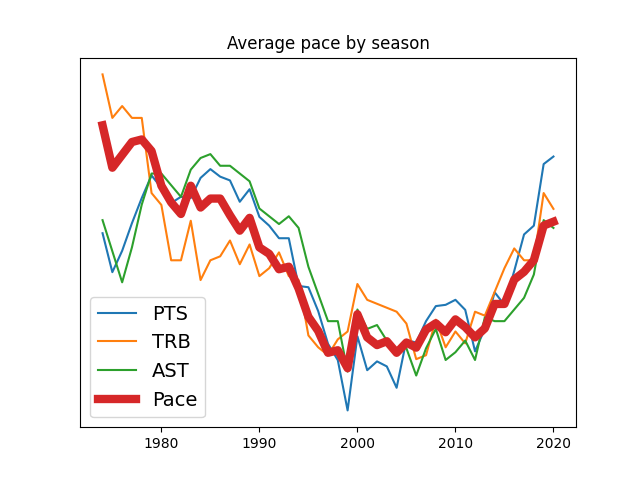
\includegraphics[scale=0.70]{pace_season.png}
\end{center}
\caption{Prosečan broj napada po 48 minuta (Pace) po sezoni}
\label{plt:pace_season}
\end{figure}

Modeli će biti trenirani na dva različita skupa podataka, jedan sadrži podatke po utakmici kao i naprednu statistiku, dok drugi, pored napredne statistike sadrži i statistiku po sto poseda. Kao što je već napomenuto, podaci sadrže ukupno 40 sezona. Ukupan broj instanci je 8295 (filtriranjem će se taj broj znatno smanjiti) dok je broj igrača koji su bili centar u najboljoj petorci lige četrdeset. Dakle, govorimo o problemu binarne klasifikacije na nebalansiranom skupu podataka.

\section{Vizuelizacija podataka}
\label{sec:vizuelizacija}

U ovoj sekciji će na grafički način biti prikazana razlika među igračima koji
su bili u prvoj petorci NBA lige, i onih koji to nisu bili. Vizuelizacija će biti
prikazana na sva tri pomenuta skupa podataka (po utakmici, po sto poseda i napredni podaci). Prikazom raspodela proverićemo da li je razlika između igrača primetna kao i to da li postoji razlika između podataka po utakmici i po posedu. Pre nego što se grafici prikažu, napomenimo da je urađeno filtriranje podataka. Izbačeni su svi igrači koji su u jednoj sezoni imali manje od 40 odigranih utakmica (od 82) i igrači koji su odigrali manje od 25 minuta po utakmici (od 48). Razlog za to će biti objašnjen u sledećoj sekciji. Na slici \ref{plt:dist_plot_pts} je prikazana raspodela po poenima po utakmici i po sto poseda, dok se na slici \ref{plt:dist_plot_per} vidi raspodela za PER statistiku.

\begin{figure}[h!]
\begin{center}
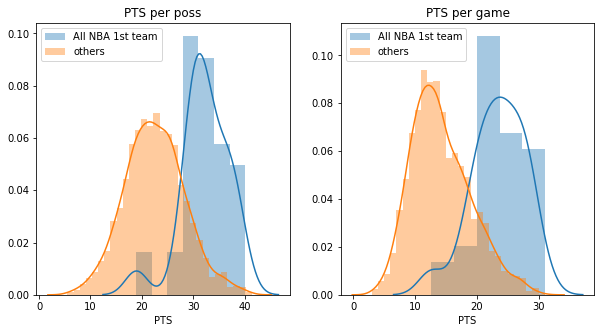
\includegraphics[scale=0.50]{dist_plot_points.png}
\end{center}
\caption{Raspodela poena po 100 poseda i po utakmici}
\label{plt:dist_plot_pts}
\end{figure}

\begin{figure}[h!]
\begin{center}
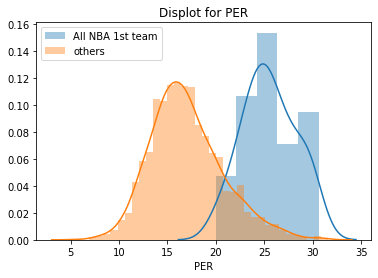
\includegraphics[scale=0.50]{dist_plot_per.png}
\end{center}
\caption{Raspodela za PER (Player Efficiency Rating)}
\label{plt:dist_plot_per}
\end{figure}

Lako se mogu primetiti razlike među vrednostima, ali ono što se ne može
primetiti odavde je razlika u broju instanci dva skupa, koja je znatna. Zbog toga
podatke prikazujemo na druge načine. Na slikama \ref{plt:swarm_plot_pts}, \ref{plt:swarm_plot_trb}, \ref{plt:swarm_plot_per} i \ref{plt:swarm_plot_bpm} se lakše primečuje razlika između instanci dve klase. Jedna tačka na slici predstavlja jednog igrača.

\begin{figure}[h!]
\begin{center}
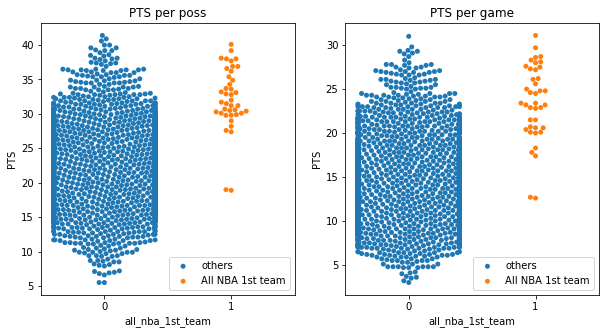
\includegraphics[scale=0.40]{swarm_plot_pts.png}
\end{center}
\caption{Poeni po 100 poseda i po utakmici}
\label{plt:swarm_plot_pts}
\end{figure}

\begin{figure}[h!]
\begin{center}
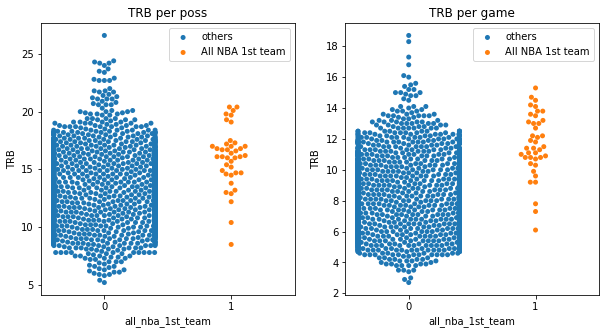
\includegraphics[scale=0.40]{swarm_plot_trb.png}
\end{center}
\caption{Skokovi po 100 poseda i po utakmici}
\label{plt:swarm_plot_trb}
\end{figure}

\begin{figure}[h!]
\begin{center}
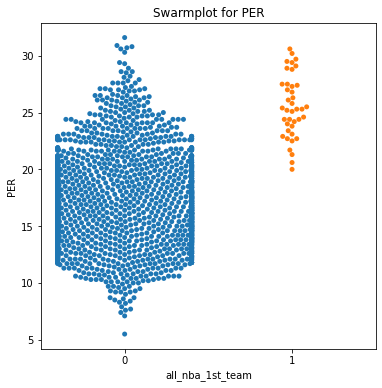
\includegraphics[scale=0.40]{swarm_plot_per.png}
\end{center}
\caption{PER}
\label{plt:swarm_plot_per}
\end{figure}

\begin{figure}[h!]
\begin{center}
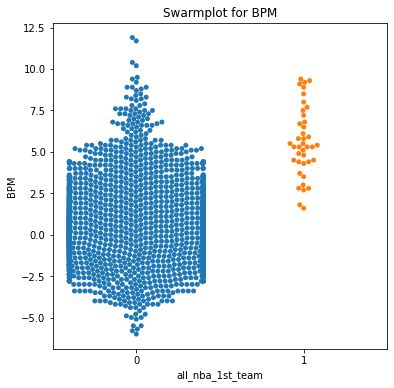
\includegraphics[scale=0.40]{swarm_plot_bpm.png}
\end{center}
\caption{BPM}
\label{plt:swarm_plot_bpm}
\end{figure}

Odavde možemo zaključiti da razlika među klasama definitivno postoji, ali
postoje igrači koji nisu bili u prvoj petorci a imaju sličnu ili čak bolju statistiku od igrača koji jesu. Sličan odnos se dobija i za ostale atribute. Ovo znači da je moguće da će modeli imati poteškoće da pravilno klasifikuju podatke. 

Posmatrajmo još i sledeće dve slike (broj \ref{plt:box_plot_pts} i \ref{plt:box_plot_ws}). One nam daju istu informaciju kao i grafici iznad, da razlika postoji u proseku ali da postoje igrači koji nisu bili u najboljoj petorci a da su to statistički zaslužili.

\begin{figure}[h!]
\begin{center}
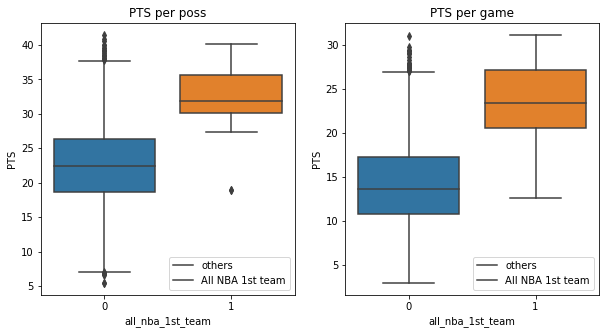
\includegraphics[scale=0.40]{box_plot_pts.png}
\end{center}
\caption{Raspodela poena po sto poseda i po utakmici}
\label{plt:box_plot_pts}
\end{figure}

\begin{figure}[h!]
\begin{center}
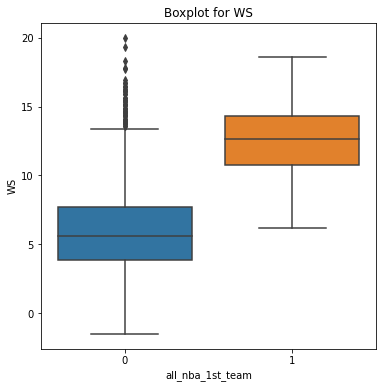
\includegraphics[scale=0.40]{box_plot_ws.png}
\end{center}
\caption{Raspodela za WS}
\label{plt:box_plot_ws}
\end{figure}

\section{Atributi}
\label{sec:atributi}

Sada se možemo okrenuti analizi atributa podataka. Kao što je već rečeno,
imamo dva csv fajla, jedan sa kombinacijom statistika po utakmici i napredim
statistikama, dok je drugi kombinacija statistike po sto poseda i naprednih statistika. Dimenzije tih csv fajlova su redom 8295x51 i 8295x52. Dakle, od 8295
igrača, samo 40 su proglašeni za startne centre (jedan po sezoni).

Prvo izbacujemo one atribute za koje ne želimo da imaju uticaj na klasifikaciju, zbog toga što ne ocenjuju igru nekog igrača. To su ime igrača (Player), tim za koji je on igrao (Tm), njegova starost (Age), pozicija na kojoj je igrao (Pos) kao i sezona u kojoj je igrao (season). 

Nakon toga proveravamo koji atributi imaju NaN vrednosti. To su GS (koji se nije
merio početkom 80ih godina), kao i razne šuterske statistike poput FG\%, 2P\%,
3P\% i FT\%. Izbacujemo svih pet atributa iz podataka. Napomenimo da nam informacije o uspešnosti šutiranja ostaju u podacima zbog toga što postoje FG i FGA atributi (i njihovi ekvivalenti za ostale vrste šuteva).

Jedan od implicitnih uslova koji moraju biti ispunjeni da bi igrač bio startni
centar je igranje određenog broja utakmica u sezoni, kao i određenog broja
minuta po utakmici. To je tako zbog toga što se za najboljeg centra lige uvek
bira veoma dobar igrač, a takav igrač je naravno bitan za svoju ekipu i zbog toga igra dosta utakmica, kao i dosta minuta po utakmici. Zbog toga poredimo prosečan broj utakmica kao i broj minuta po utakmici startnog centra i ostalih (tabela \ref{tab:g_mp}).

\begin{table}[!h]
\begin{center}
\begin{tabular}{|c|c|c|} \hline
\multicolumn{3}{|c|}{\textbf{Startni centri}} \\ \hline
\textbf{} & \textbf{Utakmice} & \textbf{Minuti} \\ \hline
Srednja vrednost & 75.4 & 36.4 \\ \hline
Minimum          & 46.0 & 30.1 \\ \hline
Maximum          & 82.0 & 42.0 \\ \hline
\multicolumn{3}{|c|}{\textbf{Ostali centri}} \\ \hline
\textbf{} & \textbf{Utakmice} & \textbf{Minuti} \\ \hline
Srednja vrednost & 48.8 & 18.6 \\ \hline
Minimum          & 1.0  & 0.0  \\ \hline
Maximum          & 85.0 & 44.5 \\ \hline
\end{tabular}
\caption{Razlika izeđu G i MP}
\label{tab:g_mp}
\end{center}
\end{table}

Na osnovu dobijenih rezultata filtriramo van podataka sve igrače koji su
odigrali ili manje od 40 utakmica u sezoni ili manje od 25 minuta po utakmici.
Nakon filtriranja izbacujemo oba ova atributa zbog toga što ne želimo da utiču
na razultat klasifikacije iz tog razloga što ne mere učinak igrača. Ovim filtiranjem
smo sveli podatke na dimenzije redom 2121x39 i 2121x40.

Sada ćemo proveriti korelacije između atributa i ciljne promenljive, kao i
između samih atributa. Kako atributa ima mnogo, nećemo prikazati korelacije
između svih njih, već između nekih odabranih.

Proverom korelacije atributa sa ciljnom promenljivom zaključujemo da ne
postoji nijedan atribut koji je visoko korelisan sa ciljnom promenljivom. Najviši
koeficijent korelacije imaju napredne statistike poput VORP, BPM i WS. Pored
njih visok stepen korelacije imaju i BLK, FG i FTA. Postoje i atributi koji
imaju veoma nizak koeficijent korelacije (između -0.1 i 0.1), poput 3PA i 3P, ali njih nećemo odstraniti.

U podacima koji su kombinacija napredne statistike i statistike po utakmici
primećujemo da su visoko korelisani sledeći atributi (koeficijent iznosi preko 0.85): TS\% i eFG\%, USG\% i FGA i PTS, TRB i TRB\%, DRB i DRB\%, ORB i ORB\%, AST i AST\%, BLK i BLK\%, WS i WS/48 i OWS, BPM i OBPM i VORP. Slične vrednosti korelacija se dobijaju i za drugu vrstu podataka, kombinaciju po sto poseda i napredne
statistike. Zbog korelisanih atributa, biće kreirane dve vrste modela, jedna sa svim atributima i druga u kojoj će biti izbačeni neki od njih.

Za sam kraj ćemo RFE metodom ispitati koji atributi su najbitniji za klasi-
fikaciju. Model koji će biti korišćen za RFE je RandomForest i biće izabrano 20
najbitnijih atributa. Zbog nebalansiranosti podataka RFE će biti pokrenut za tri metode balansiranja podataka, nasumično smanjivanje broja instanci veće klase, nasumično povećavanje broja instanci manje klase kao i SMOTE. Rezultati su prikazani u nastavku, prvo za kombinaciju naprednih i po utakmici podataka a nakon toga i za kombinaciju naprednih i po sto poseda.

\begin{center}
\line(1,0){250}
\end{center}

\begin{itemize}
	\item \textbf{Undersampling} 2P, FT, FTA, TRB, BLK, TOV, PTS, PER, FTr,
DRB\%, TRB\%, AST\%, BLK\%, USG\%, DWS, WS, WS/48, DBPM, BPM,
VORP
	\item \textbf{Oversampling} FG, 2P, eFG\%, FT, FTA, AST, BLK, TOV, PTS, PER,
3PAr, FTr, AST\%, BLK\%, USG\%, DWS, WS, WS/48, BPM, VORP
	\item \textbf{SMOTE} 2PA, eFG\%, FT, FTA, BLK, TOV, PTS, PER, TS\%, AST\%,
BLK\%, USG\%, OWS, DWS, WS, WS/48, OBPM, DBPM, BPM, VORP
\end{itemize}

\begin{center}
\line(1,0){250}
\end{center}

\begin{itemize}
	\item \textbf{Undersampling} FG, 2P, FT, FTA, DRB, TRB, TOV, PTS, DRtg, PER,
FTr, ORB\%, USG\%, OWS, DWS, WS, WS/48, DBPM, BPM, VORP
	\item \textbf{Oversampling} FG, 2P, FT, FTA, AST, BLK, TOV, PTS, DRtg, PER,
TS\%, 3PAr, AST\%, BLK\%, USG\%, DWS, WS, WS/48, BPM, VORP
	\item \textbf{SMOTE} FG, 2P, FT, FTA, BLK, TOV, PTS, ORtg, DRtg, PER, TS\%,
FTr, BLK\%, USG\%, DWS, WS, WS/48, OBPM, BPM, VORP
\end{itemize}

\begin{center}
\line(1,0){250}
\end{center}

Važnost atributa je slična za sve isprobane modele. Primetimo i to da su obične statistike važnije od naprednih, što možda nije očekivano.

\section{Modeli}
\label{sec:modeli}

U ovoj sekciji ćemo kreirati modele nad podacima i evaluirati ih. Kako je
skup podataka nebalansiran, tačnost (accuracy) nam neće biti od značaja, tako
da će se više pažnje obratiti na druge metrike poput odziva (recall) i preciznosti
(precision). Takođe, da bi se ta nebalansiranost zaobišla, biće korišćena \textit{imblearn} biblioteka uz pomoć koje ćemo kontrolistati balansiranost.

Modeli koji će biti trenitani nad podacima su takvi da podržavaju verovatnoće i to su:
\begin{itemize}
	\item Support Vector Machine (\textbf{SVM})
	\item Random Forest (\textbf{RFC})
	\item Gradient Boosting (\textbf{GBC})
\end{itemize}

Podsetimo se da imamo dva skupa podataka, dimenzija redom 2121x39 i
2121x40. Modeli će biti trenirani i na podacima sa uklonjenim određenim atributima (koji su visoko korelisani među sobom). Njihove dimenzije su redom 2121x28 i 2121x30. Od 2121 instance, 40 pripada centru koji je bio član prve petorke NBA lige.

Pre treniranja, delimo podatke na trening i test skupove. Izabrano je da je
veličina test skupa 0.33 veličine podataka, dok trening skup čini ostatak. Pri
podeli uzeta je u obzir raspodela klasa (stratifikacija). Rezultat je da trening skup ima 27 instanci centara prvog tima i 1394 instance ostalih, dok test skup ima redom 13 i 687 primeraka. Nakon podele na trening i test, podaci su standardizovani korišćenjem sklearn biblioteke.

Da bismo smanjili preprilagođavanje, kreirano je nekoliko modela sa različitim parametrima korišćenjem GridSearchCV metoda. Veličina skupa za validaciju je 10 dok je metrika koja se maksimizuje \textbf{odziv} iz tog razloga što nam je cilj da ispravno pogodimo instance pozitivne klase.

GridSearch je pokrenut nad različitim skupovima podataka, na skupu bez
balansiranja klasa (odnos klasa na trening skupu je 1394 prema 27), na skupu
gde je broj primeraka veće klase smanjen u odnosu 1:4 (odnos klasa na trening
skupu je 108 prema 27), na skupu gde je broj primeraka manje klase uvećan u
odnosu 1:4 (odnos klasa na trening skupu je 1394 prema 348) i na skupu gde
imamo isti broj instanci obe klase (odnos na trening skupu je 1394 prema 1394).
Naravno, svi ovi modeli se testiraju nad istim test skupom.

Kako imamo četiri vrste podataka nad kojim treniramo modele, tri modela
kao i četiri načina na koji su klase balansirane, kreirano je ukupno 48 modela. U
nastavku će detaljnije biti prikazano samo nekoliko najboljih od njih. Za evaluaciju svakog od modela će se koristiti preciznost, odziv, f1 skor, log loss i površina ispod ROC krive.

\subsection{Modeli sa svim atributima}
\label{subsec:svi_atributi}

Kako imamo dve različite vrste podataka, podelićemo ovu sekciju na dva dela. Napomenimo još jednom da je svaki model takav da maksimizuje odziv i smanjuje preprilagođavanje što je više moguće.

\subsubsection{Kombinacija podataka po utakmici i naprednih podataka}
\label{subsubsec:kombo_pg_adv}

Dakle, zbog nebalansiranosti podataka isprobano je nekoliko strategija. Prva
je bila da se skup za trening ne menja. Ovaj pristup nije doveo do baš dobrih
rezultata. Najbolje rezultate od svih modela na ovom skupu ima SVM kome je
odziv za pozitivnu klasu na test skupu 0.38, preciznost 0.42, dok mu površina
ispod ROC krive iznosi 0.69.

Nakon ovoga, promenjen je skup za trening na takav način da je broj instanci
veće klase smanjen (undersampling) i ovaj pristup je doveo do modela koji imaju dobre rezultate (tabela \ref{tab:undersampling_pg}). Prikazane metrike, preciznost, odziv i f1 skor se odnose na pozitivnu klasu, a ne na prosek modela.

\begin{table}[!h]
\begin{center}
\begin{tabular}{|c|c|c|c|c|c|} \hline
\textbf{Model} & \textbf{Preciznost} & \textbf{Odziv} & \textbf{f1 skor} & \textbf{Roc auc} & \textbf{Log loss} \\ \hline
svm & 0.21 & 0.92 & 0.34 & 0.93 & 0.13 \\ \hline
rfc & 0.27 & 0.85 & 0.41 & 0.90 & 0.11 \\ \hline
gbc & 0.24 & 0.92 & 0.39 & 0.93 & 0.26 \\ \hline
\end{tabular}
\caption{Rezultati undersampling modela}
\label{tab:undersampling_pg}
\end{center}
\end{table}

Vidimo da sva tri modela imaju visok odziv, kao i visoku vrednosti za površinu ispod ROC krive. Preciznost za sva tri modela je niska, što može predstavljati potencijalni problem. Napomenimo i to da su modeli upoređeni sa nasumičnim klasifikatorom (Dummy) i da imaju znatno bolje rezultate od njega.

Modeli kreirani nad trening skupom kome je dodato još primeraka manje
klase na nasumičan način nemaju dobre rezultate. Štaviše, dobijeni rezultati
su veoma slični rezultatima modela na kojima nije izvršeno balansiranje klasa,
osim za SVM model koji je bolji i koji za pozitivnu klasu ima preciznost 0.41,
odziv 0.69, f1 skor 0.51 dok mu je površina ispod ROC krive 0.84.

Poslednja metoda je SMOTE uz pomoć koje je izjednačen broj instanci za obe klase na
trening skupu. Dobijeni rezultati se mogu pronaći u tabeli \ref{tab:smote_pg}. Kao i u prethodnoj tabeli, preciznost, odziv i f1 skor važe samo za pozitivnu klasu.

\begin{table}[!h]
\begin{center}
\begin{tabular}{|c|c|c|c|c|c|} \hline
\textbf{Model} & \textbf{Preciznost} & \textbf{Odziv} & \textbf{f1 skor} & \textbf{Roc auc} & \textbf{Log loss} \\ \hline
svm & 0.20 & 0.85 & 0.33 & 0.89 & 0.13 \\ \hline
rfc & 0.38 & 0.77 & 0.51 & 0.87 & 0.07 \\ \hline
gbc & 0.33 & 0.23 & 0.27 & 0.61 & 0.18 \\ \hline
\end{tabular}
\caption{Rezultati SMOTE modela}
\label{tab:smote_pg}
\end{center}
\end{table}

Lako primećujemo da GBC model ne daje dobre rezultate, dok su rezultati
za druga dva zadovoljavajući, iako je preciznost niska. Sva tri modela imaju
bolji rezultat od nasumičnog klasifikatora.

Sada ćemo proveriti kako modeli klasifikuju igrače iz sezone 2019-20. Izabrana su četiri igrača za koje se smatra da su glavni kandidati za najboljeg centra lige. To su Anthony Davis, Joel Embiid, Rudy Gobert i Nikola Jokić. Pogledajmo sledeću tabelu (slika \ref{plt:clf_pg}). Za svakog igrača je prikazana verovatnoća da postane najbolji centar za odabranih pet modela. Ti modeli su sva tri modela trenirana na skupu u kome je broj instanci veće klase smanjen kao i dva bolja modela trenirana na skupu dobijenom SMOTE metodom, SVM i RFC. Pored tih rezultata, prikazan je i njihov prosek.

\begin{figure}[h!]
\begin{center}
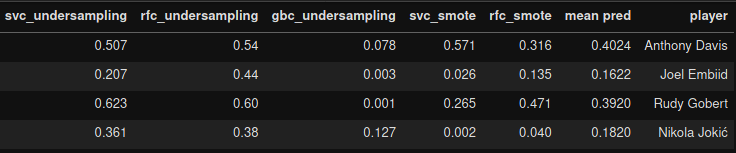
\includegraphics[scale=0.50]{clf_pg.png}
\end{center}
\caption{Verovatnoće da igrač bude u prvoj petorci za svaki model}
\label{plt:clf_pg}
\end{figure}

Razlika između prvog i drugog mesta nije velika. Modeli najveću šansu daju
Dejvisu, pa nakon toga Goberu. Zanimljive su verovatnoće GBC modela treniranog nad samplovanim podacima, koji svakom igraču ne daje skoro nikakve šanse da se nađe u startnoj petorci, osim Jokiću koga ostali klasifikatori ne cene.

\subsubsection{Kombinacija podataka po sto poseda i naprednih podataka}
\label{subsubsec:kombo_pp_adv}

Pogledajmo sada da li će se pojaviti neka razlika nad podacima po posedu,
koji bi trebalo da bolje skaliraju različite sezone. Već u rezultatima modela
koji su trenirani nad nebalansiranim podacima se primećuje razlika, gde SVM i
GBC daju malo bolje rezultate nego za podatke po utakmici. Najbolji od njih je
ponovo SVM sa sledećim vrednostima za pozitivnu klasu: odziv 0.46, preciznost
0.50, f1 skor 0.48 i površina ispod ROC krive 0.73.

I za ove podatke modeli koji su trenirani kada se broj instanci veće klase smanji daju dobre rezultate. Oni su prikazani u tabeli broj \ref{tab:undersampling_pp}. Vrednosti preciznosti, odziva i f1 skora su prikazani samo za pozitivnu klasu.

\begin{table}[!h]
\begin{center}
\begin{tabular}{|c|c|c|c|c|c|} \hline
\textbf{Model} & \textbf{Preciznost} & \textbf{Odziv} & \textbf{f1 skor} & \textbf{Roc auc} & \textbf{Log loss} \\ \hline
svm & 0.18 & 0.92 & 0.31 & 0.92 & 0.13 \\ \hline
rfc & 0.33 & 0.92 & 0.49 & 0.94 & 0.10 \\ \hline
gbc & 0.30 & 0.69 & 0.42 & 0.83 & 0.08 \\ \hline
\end{tabular}
\caption{Rezultati undersampling modela}
\label{tab:undersampling_pp}
\end{center}
\end{table}

Vidimo da SVM i RFC daju visoke vrednosti odziva ali imaju nisku preciznost, što se u većoj meri odnosi na SVM. Model GBC daje malo slabije rezultate u globalu, ali i malo veću preciznost od SVM modela. Svaki od ovih modela daje bolje rezultate od nasumičnog (Dummy) klasifikatora.

Rezultati modela nad podacima na kojima je broj instanci manje klase uvećan su lošiji od prethodnih i sva tri modela na test skupu imaju vrednost odziva 0.31 za pozitivnu klasu. Takođe imaju i gotovo identičnu površinu ispod ROC krive koja iznosi približno 0.65 za svaki model.

Modeli trenirani nad podacima dobijenim SMOTE metodom su lošiji od onih koji su trenirani nad podacima koji sadrže statistiku po utakmici. Najbolji od njih je RFC kome je odziv za pozitivnu klasu 0.69, preciznost 0.39 a f1 skor 0.50. Površina ispod ROC krive je 0.84 dok je log loss 0.07. Ostala dva modela imaju znatno lošije rezultate.

Sada ćemo, kao i u prethodnoj sekciji izabrati najbolje modele i prikazati njihove rezultate za ista četiri igrača iz sezone 2019-20 (slika \ref{plt:clf_pp}).

\begin{figure}[h!]
\begin{center}
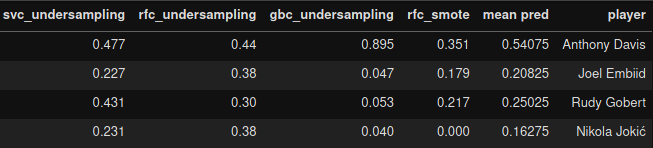
\includegraphics[scale=0.50]{clf_pp.png}
\end{center}
\caption{Verovatnoće da igrač bude u prvoj petorci za svaki model}
\label{plt:clf_pp}
\end{figure}

Prva dva mesta zauzimaju isti igrači samo je razlika znatno veća. Ovi modeli ne samo da daju veću verovatnoću Dejvisu, nego daju i manju verovatnoću Goberu. Jokić i Embiid su zamenili mesta. Zanimljive su verovatnoće GBC modela koji je gotovo siguran da će Dejvis biti startni centar, dok ostale igrače ne ceni ni malo i ne daje im skoro nikakvu šansu.


\subsection{Modeli sa manjim brojem atributa}
\label{subsec:manje_atributa}

Sada ćemo proveriti kakve rezultate daju modeli koji su trenirani nad jednostavnijim podacima, tačnije podacima sa nekoliko uklonjenih atributa koji su visoko korelisani među sobom. Kod obe vrste podataka ukljonjeni su isti atributi. Atribut USG\% je uklonjen zbog toga što je visoko korelisan i sa PTS i sa FGA. Iz istog razloga uklanjamo TRB\% (sa TRB), ORB\% (sa ORB), DRB\% (sa DRB), AST\% (sa AST), STL\% (sa STL) i BLK\% (sa BLK). Od naprednih statistka visoko korelisane među sobom su WS i WS/48, pa zbog toga izbacujemo drugu. Takođe, WS i OWS imaju visok koeficijent korelacije te se izbacuje i OWS. Na kraju, izbacuje se još i OBPM zbog visoke korelisanosti sa BPM. Napomenimo da DWS i WS kao i DBPM i BPM nemaju veoma visok stepen korelacije. Iz skupa koji predstavlja podatke po utakmici izbacuje se još i TS\% atribut, zbog toga što je visoko korelisan sa eFG\%. Taj atribut se ne izbacuje iz podataka po posedu zbog toga što kod njih eFG\% ne postoji.

Time su dobijena dva nova skupa podataka manjih dimenzija. Dimenzije kombinacije podataka po utakmici i naprednih su 2121x28 dok su dimenzije drugog skupa podataka 2121x30.

\subsubsection{Kombinacija podataka po utakmici i naprednih podataka}
\label{subsubsec:kombo_pg_adv_simple}

Kao i kod modela sa više atributa, rezultati modela treniranih nad nebalansiranim podacima nisu zadovoljavajući. Najbolje se pokazao SVM model, dok ostala dva imaju znatno lošije rezultate.

Modeli nastali nad podacima kojima je broj instanci veće klase smanjen imaju, ponovo, kao i kod podataka sa svim atributima, veoma dobre rezultate odziva na test skupu (tabela \ref{tab:undersampling_pg_simple}), iako im preciznost nije visoka. Odziv, preciznost i f1 skor su prikazani za pozitivnu klasu.

\begin{table}[!h]
\begin{center}
\begin{tabular}{|c|c|c|c|c|c|} \hline
\textbf{Model} & \textbf{Preciznost} & \textbf{Odziv} & \textbf{f1 skor} & \textbf{Roc auc} & \textbf{Log loss} \\ \hline
svm & 0.21 & 0.92 & 0.34 & 0.93 & 0.12 \\ \hline
rfc & 0.29 & 1.00 & 0.45 & 0.98 & 0.11 \\ \hline
gbc & 0.26 & 0.85 & 0.39 & 0.90 & 0.17 \\ \hline
\end{tabular}
\caption{Rezultati undersampling modela}
\label{tab:undersampling_pg_simple}
\end{center}
\end{table}

Kada uporedimo ove modele sa onim treniranim nad istim podacima, ali bez
uklanjanja atributa, primećujemo da imaju slične rezultate. Neke vrednosti su
malo niže, dok su neke malo više, zavisno od modela. Jedino poboljšanje koje se primećuje kod sva tri modela je veća površina ispod ROC krive, ali razlika nije
velika.

Kod podataka sa svim atributima, modeli nisu dali zadovoljavajuće rezultate
na test skupu kada se uveća broj instanci manje klase. Ovde to nije slučaj za
svaki model. Pogledajmo tabelu \ref{tab:oversampling_pg_simple}.

\begin{table}[!h]
\begin{center}
\begin{tabular}{|c|c|c|c|c|c|} \hline
\textbf{Model} & \textbf{Preciznost} & \textbf{Odziv} & \textbf{f1 skor} & \textbf{Roc auc} & \textbf{Log loss} \\ \hline
svm & 0.48 & 0.77 & 0.59 & 0.88 & 0.06 \\ \hline
rfc & 1.00 & 0.38 & 0.56 & 0.69 & 0.04 \\ \hline
gbc & 0.50 & 0.15 & 0.24 & 0.58 & 0.08 \\ \hline
\end{tabular}
\caption{Rezultati oversampling modela}
\label{tab:oversampling_pg_simple}
\end{center}
\end{table}

Primetimo da SVM klasifikator ima visoku vrednost odziva za pozitivnu klasu. Pored toga, u odnosu na prehodni SVM model, ima višu vrednost za preciznost i f1 skor. Ostala dva modela nisu toliko dobra, pogotovu GBC koji sudeći prema površini ispod ROC krive ima poteškoća da uopšte razlikuje klase.

Rezultati modela nad podacima samplovanim SMOTE metodom (tabela \ref{tab:smote_pg_simple}) su uglavnom u redu. GBC klasifikator ima nisku vrednost odziva, pa neće biti razmatran u nastavku. Ponovo SVM ima najveću vrednost odziva, ali isto tako i nisku preciznost.

\begin{table}[!h]
\begin{center}
\begin{tabular}{|c|c|c|c|c|c|} \hline
\textbf{Model} & \textbf{Preciznost} & \textbf{Odziv} & \textbf{f1 skor} & \textbf{Roc auc} & \textbf{Log loss} \\ \hline
svm & 0.19 & 0.85 & 0.31 & 0.89 & 0.16 \\ \hline
rfc & 0.36 & 0.69 & 0.47 & 0.83 & 0.06 \\ \hline
gbc & 0.44 & 0.31 & 0.36 & 0.65 & 0.08 \\ \hline
\end{tabular}
\caption{Rezultati SMOTE modela}
\label{tab:smote_pg_simple}
\end{center}
\end{table}

Proverimo sada verovatnoće da igrač bude član najbolje petorke najboljih modela za ista četiri igrača kao i ranije (slika \ref{plt:clf_pg_simpler}). Rezultati su slični u smislu da modeli mnogo veće šanse daju Dejvisu i Goberu nego Jokiću i Embiidu, s tim da je Gober sada na prvom mestu u proseku iako i dalje postoje modeli koji više cene Dejvisa. Primetimo da SVM model nastao povećavanjem broja uzoraka manje klase daje nisku verovatnoću za prvu petorku svakom igraču, što je interesantno. Bez njega, prosek verovatnoća je sledeći: Gobert - 0.466, Davis - 0.309, Jokić - 0.160 i Embiid - 0.087. Raspored je ostao isti ali su verovatnoće realnije.

\begin{figure}[h!]
\begin{center}
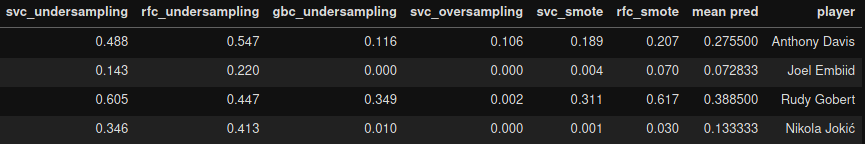
\includegraphics[scale=0.50]{clf_pg_simpler.png}
\end{center}
\caption{Verovatnoće da igrač bude u prvoj petorci za svaki model}
\label{plt:clf_pg_simpler}
\end{figure}

\subsubsection{Kombinacija podataka po sto poseda i naprednih podataka}
\label{subsubsec:kombo_pp_adv_simple}

Za sam kraj, videćemo kako se ponašaju modeli nad skupom podataka u kome se nalaze statistike po sto poseda ali sa manje atributa. Ovi modeli prate skoro isti princip kao i ostali, gde rezultati nad podacima bez balansiranja nisu zadovoljavajući. Isto se može reći i za modele trenirane nad podacima gde je manja klasa uvećana. Modeli gde je smanjen broj instanci veće klase su dobri i prikazani su u tabeli \ref{tab:undersampling_pp_simple}. Kod modela treniranih nad podacima koji su balansirani SMOTE metodom najbolji je RFC dok su ostala dva lošija.

\begin{table}[!h]
\begin{center}
\begin{tabular}{|c|c|c|c|c|c|} \hline
\textbf{Model} & \textbf{Preciznost} & \textbf{Odziv} & \textbf{f1 skor} & \textbf{Roc auc} & \textbf{Log loss} \\ \hline
svm & 0.18 & 0.92 & 0.31 & 0.92 & 0.13 \\ \hline
rfc & 0.25 & 1.00 & 0.41 & 0.97 & 0.12 \\ \hline
gbc & 0.33 & 1.00 & 0.50 & 0.98 & 0.14 \\ \hline
\end{tabular}
\caption{Rezultati undersampling modela}
\label{tab:undersampling_pp_simple}
\end{center}
\end{table}

Kao što se iz tabele može primetiti, modeli GBC i RFC imaju veoma dobre rezultate na test skupu kao i veoma visoke površine ispod ROC krive. SVM model daje malo lošije rezultate, ali svakako dobre. Proverimo sada verovatnoće predviđanja ovih modela za ista četiri igrača (slika \ref{plt:clf_pp_simpler}).

\begin{figure}[h!]
\begin{center}
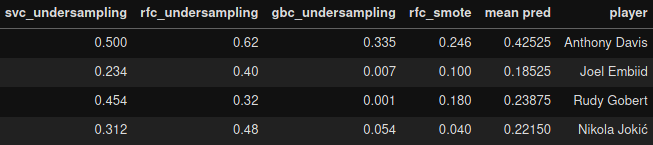
\includegraphics[scale=0.50]{clf_pp_simpler.png}
\end{center}
\caption{Verovatnoće da igrač bude u prvoj petorci za svaki model}
\label{plt:clf_pp_simpler}
\end{figure}

Ovi modeli takođe najviše cene Dejvisa koji ima skoro duplo veću verovatnoću od drugoplasiranog Gobera. Šanse za ostala tri centra su približnih vrednosti. Ovi modeli više cene Jokića i Embiida od prethodnih, ali im i dalje ne daju velike šanse.

\subsection{Zašto modeli predviđaju ono što predviđaju}
\label{subsec:modeli_pred}

Na samom kraju prikazujemo SHAP vrednosti za neke od modela. SHAP nam govori koji atributi su najznačajniji prilikom klasifikacije. Prikazujemo važnost svakog atributa za model SVM napravljen undersamplingom nad podacima po posedu sa svim (slike \ref{plt:shap_1} i \ref{plt:shap_2}) i nad podacima sa odstranjenim atributima (slika \ref{plt:shap_simple_1} i \ref{plt:shap_simple_2}).

\begin{figure}[h!]
\begin{center}
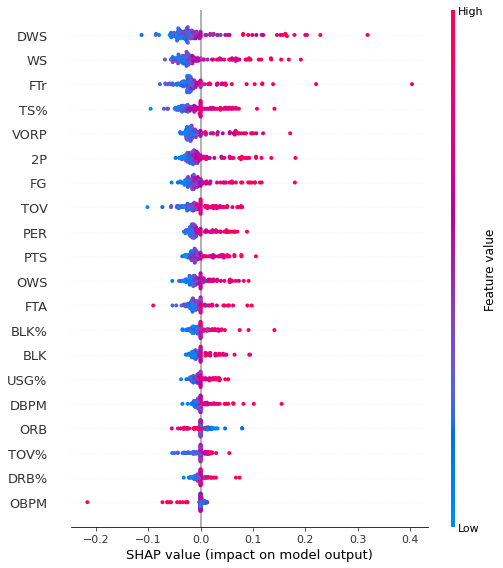
\includegraphics[scale=0.4]{shap_1.png}
\end{center}
\caption{Značaj atributa za svaku instancu}
\label{plt:shap_1}
\end{figure}

\begin{figure}[h!]
\begin{center}
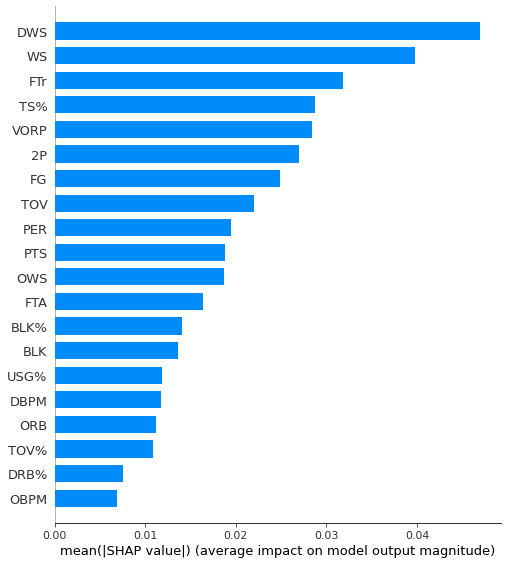
\includegraphics[scale=0.4]{shap_2.png}
\end{center}
\caption{Značaj atributa u proseku}
\label{plt:shap_2}
\end{figure}

\begin{figure}[h!]
\begin{center}
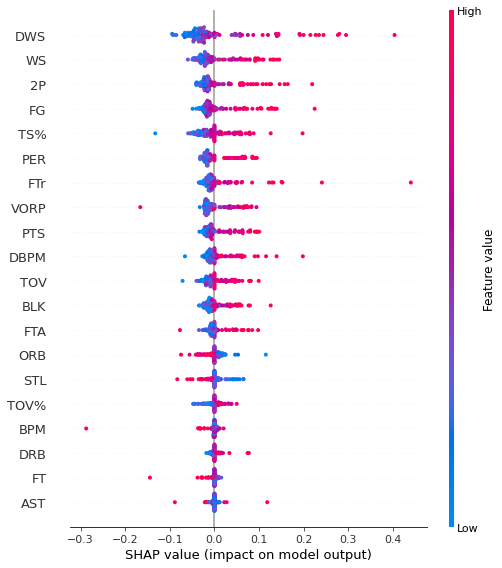
\includegraphics[scale=0.4]{shap_simple_1.png}
\end{center}
\caption{Značaj atributa za svaku instancu}
\label{plt:shap_simple_1}
\end{figure}

\begin{figure}[h!]
\begin{center}
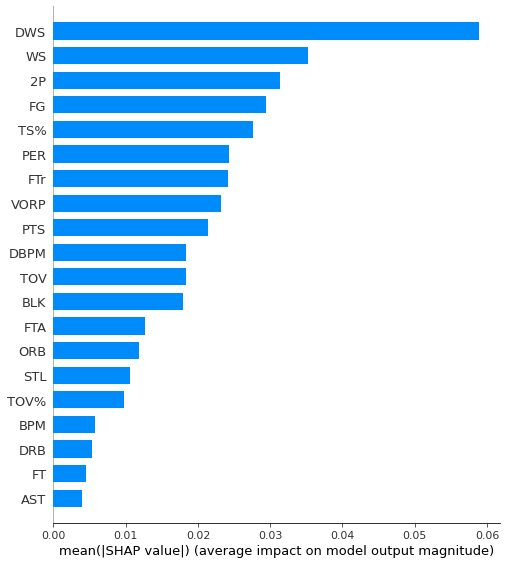
\includegraphics[scale=0.4]{shap_simple_2.png}
\end{center}
\caption{Značaj atributa u proseku}
\label{plt:shap_simple_2}
\end{figure}

Primećujemo da modeli najviše cene napredne statistike, kao i šutiranje na koš. Zanimljivo je što skokovi (TRB, ORB, DRB itd.) nisu značajniji s obzirom na to da ipak klasifikujemo centre kojima je to jedan od glavnih poslova dok su u igri. SHAP vrednosti za ostale modele se mogu pogledati na github repozitorijumu projekta.

\section{Zaključak}
\label{sec:zakljucak}

Isproban je veliki broj modela nad različitim skupovima podataka. Dobijeni rezultati su interesantini ali ne uzimaju u obzir sve kriterijume za proglašenje nekoga najboljim centrom lige, pošto je te kriterijume gotovo nemoguće definisati, već samo statistiku. Prema ovim modelima, centar koji će biti član najbolje petorke NBA lige za sezonu 2019-20 je Entoni Dejvis, dok pored njega nekoliko modela daje visoku verovatnoću i Goberu. Prema modelima, Jokić i Embiid nemaju velike šanse.

\pagebreak

\addcontentsline{toc}{section}{References}
\appendix
\bibliography{ref}
\bibliographystyle{unsrt}
\appendix

\end{document}
